\chapter{Implementacja}
W rozdziale tym przedstawiona zostanie implementacja opisanych w poprzednich
rozdziałach technik symulacji ciała miękkiego. Na implementację składają się dwa
główne komponenty - biblioteka programistyczna oraz aplikacja demonstracyjna.
Biblioteka programistyczna jest odpowiedzialna za symulację ciała miękkiego.
Stworzenie jej miało na celu ułatwienie ponownego
wykorzystania zaimplementowanych klas i umożliwienie jej samodzielnego
rozwijania w przyszłości.

Bibliotekę można skompilować w wersji tylko na CPU oraz ze wsparciem dla technologii
CUDA.  Proces ten jest automatyczny i wspierany przez użyty w projekcie program
CMake, służący do zarządzania kompilacją programu. W przypadku gdy w systemie
zostaną wykryte wymagane biblioteki oraz kompilator CUDA, nastąpi kompilacja
dodatkowych plików źródłowych.

Program CMake jest wieloplatformowy, co oznacza, że dostępne są jego wersje na
najpopularniejsze obecnie systemy operacyjne takie jak Windows, Linux czy Os X.
CMake potrafi generować pliki z regułami kompilacji dla konkretnego środowiska
deweloperskiego. Dla platformy Linux będą to skrypty \texttt{Makefile},
	natomiast dla Windows pliki projektowe \texttt{Microsoft Visual Studio}.
	Zastosowanie CMake pozwala w wygodny sposób udostępniać projekt na różne
	platformy.

% opengl
Zarówno biblioteka jak i aplikacja demonstracyjna wymagają do uruchomienia
biblioteki OpenGL w wersji minimalnie 3.3. Jest ona wymagana do uruchomienia
zaimplementowanych w bibliotece vertex, pixel i geometry shaderów. Do implementacji obliczeń
na procesorze graficznym użyto CUDA-SDK w wersji 5.5.

W implementacji wykorzystano też dwie pomocnicze biblioteki.
Pierwszą jest GLM (OpenGL Math), dostarczająca implementację wielu podstawowych
typów niezbędnych w grafice trójwymiarowej, takich jak wektor czy macierz oraz
operacji takich jak np. iloczyn skalarny czy wektorowy. Największą zaletą
biblioteki GLM jest fakt, że składa się ona tylko z plików nagłówkowych. Nie ma
zatem potrzeby wymagania jej przy procesie kompilacji czy budowania jej razem z
projektem. Wszystkie potrzebne funkcje są bezpośrednio załączane do kodu
biblioteki w momencie kompilacji.

Kolejną zaletą biblioteki GLM jest jej kompatybilność z technologią CUDA. W przypadku
gdy plik nagłówkowy biblioteki jest przetwarzany przez preprocesor kompilatora
nvcc, zdefiniowane tam makra są rozwijane na charakterystyczne dla nvcc
atrybuty kompilatora, takie jak \texttt{\_\_device\_\_} czy \texttt{\_\_host\_\_}.
W przypadku gdy użyty jest inny kompilator biblioteka GLM wykorzystuje inne
atrybuty. Umożliwia to zadeklarowanie jednej funkcji która może być użyta zarówno
w kodzie wykonywanym na GPU, jak również na CPU.

Drugą wykorzystaną biblioteką jest OpenGL Framework (GLFW) stanowiąca warstwę
abstrakcji nad natywny system zarządzania oknami oraz zdarzeniami z klawiatury i
myszki. Dostarcza też mechanizm pętli głównej niezbędny do stworzenia
interaktywnych aplikacji.

\section{Aplikacja demonstracyjna}
\subsection{Przewodnik}
Aplikacja demonstracyjna jest prostą aplikacją ze sterowaniem klawiaturowym. Po
uruchomieniu główny plan zajmuje pusta trójwymiarowa scena. Nawigacja w
aplikacji obydwa się za pośrednictwem prawego klawisza myszy i przemieszczenia
kursora. Użytkownik jest w stanie obracać się punktu
centralnego sceny oraz przybliżać się i oddalać od niego używając kółka myszki.

\begin{figure}[H]
\centering
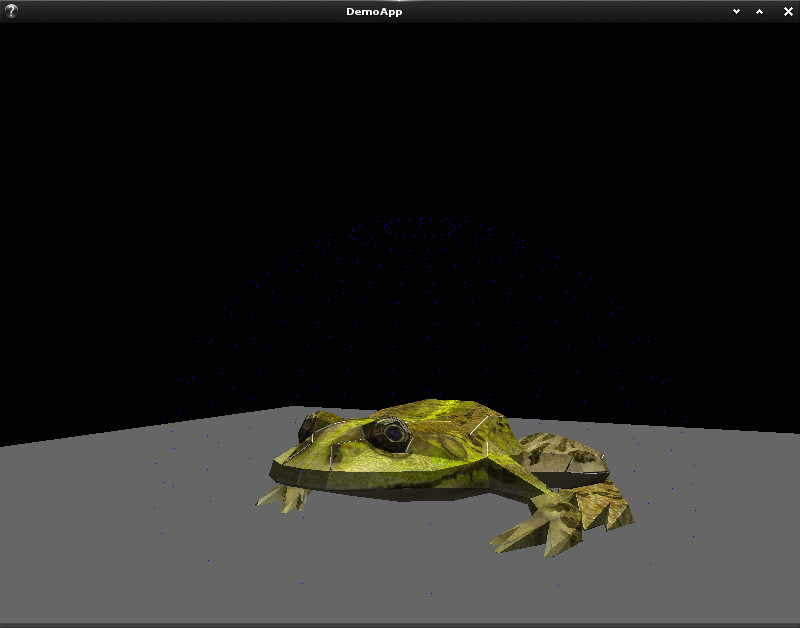
\includegraphics[scale=0.5]{images/z1.jpg}
\caption{Charakterystyki procesorów firmy Intel na przestrzeni 40 lat. Źródło: http://www.gotw.ca/}
\end{figure}

Aby zainicjować symulację należy użyć klawisza "t". Zostanie w ten sposób
stworzony model żaby, której model na licencji Royality Free
dostępny jest na stronie http://www.turbosquid.com/FullPreview/Index.cfm/ID/589370.

\begin{figure}[H]
\centering
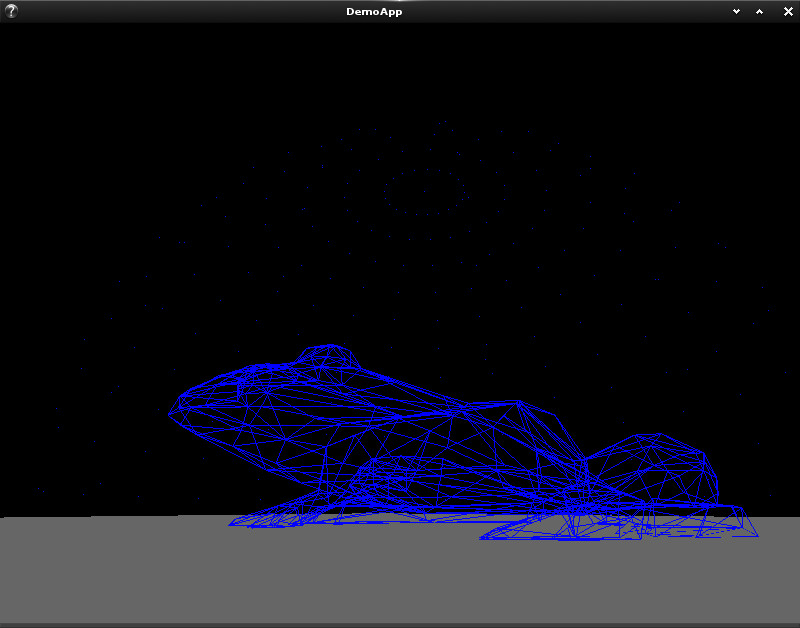
\includegraphics[scale=0.5]{images/z2.jpg}
\caption{Charakterystyki procesorów firmy Intel na przestrzeni 40 lat. Źródło: http://www.gotw.ca/}
\end{figure}

Program demonstracyjny posiada dwa tryby renderowania. W pierwszym wyświetlany
jest cały oteksturowany model wraz z oświetleniem, w drugim zaś renderowana jest
tylko siatka połączeń między wierzchołkami tworzącymi trójkąty. Aby przełączać
się między dwoma trybami należy użyć klawisza "m".

\begin{figure}[H]
\centering
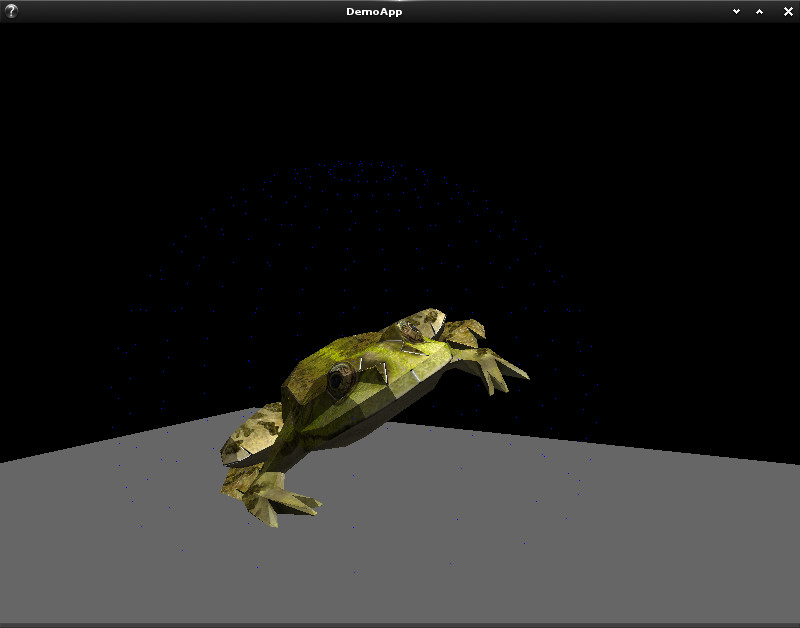
\includegraphics[scale=0.5]{images/z3.jpg}
\caption{Charakterystyki procesorów firmy Intel na przestrzeni 40 lat. Źródło: http://www.gotw.ca/}
\end{figure}

W stworzonej aplikacji istnieje możliwość interakcji z symulowanym ciałem
miękkim. W tym celu należy najechać myszą na obszar zajmowany przez model a
następnie nacisnąć i trzymać lewy przycisk myszy.

\begin{figure}[H]
\centering
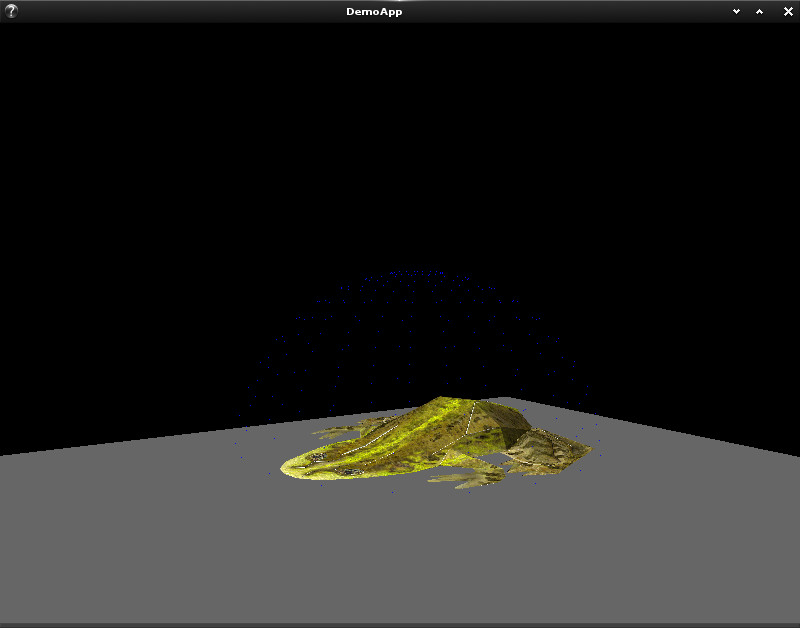
\includegraphics[scale=0.5]{images/z5.jpg}
\caption{Charakterystyki procesorów firmy Intel na przestrzeni 40 lat. Źródło: http://www.gotw.ca/}
\end{figure}

Możliwe jest również zmienianie współczynnika sprężystości symulowanego ciała. W
przypadku gdy jest on większy symulowane ciało zachowywać się będzie bardziej
jak bryła sztywna, natomiast dla małych wartości ciało wskazywać będzie zanik
wszelkich sił wewnętrznych. Zmiana sił sprężystości możliwa jest poprzez
klawisze '-' i '+'.

% GLWF
\subsection{Rysowanie okna}
W celu stworzenia okna aplikacji posłużono się open-sourcową biblioteką GLFW. Z
racji, że biblioteka te udostępnia interfejsy programisty napisane tylko w języku C
utworzona została klasa \texttt{GLFWApplication} opakowująca API biblioteki
GLFW (ang. wrapper). Oprócz zwykłego udostępniania metod, klasa ta spełnia
jeszcze dodatkowe funkcje. Udostępnia ona wirtualne metody \texttt{OnRender}
oraz \texttt{OnUpdate}, które będą wykorzystywane odpowiednio przy rysowaniu
ramki obrazu oraz przy symulacji fizyki. Dodatkowo klasa GLFWApplication rejestruje wszystkie błędy zgłaszane przez
GLFW i drukuje je do standardowego wyjścia błędów.

% statyczny krok symulacji
\subsection{Krok symulacji}
Kolejnymi funkcjonalnościami dostarczanymi przez klasę \texttt{GLFWApplication} jest
uruchomienie pętli głównej aplikacji oraz wywoływanie metod \texttt{OnUpdate} oraz \texttt{OnRender}.
Jest to niezbędne w celu zsynchronizowania odświeżania obrazu i
symulacji fizyki. Pętla główna zdefiniowana na listingu (\ref{main_loop})
pozwala na użycie stałego kroku czasu w symulacji fizyki przy jednoczesnym
zachowaniu możliwości odświeżania obrazu w różnej częstotliwości. Przyjęcie
stałego kroku czasu jest niezbędne w symulacji ponieważ
techniki w niej zaimplementowane są wrażliwe na jego zmianę, czego efektem jest
np. zmiana sztywności ciała obserwowana przy zmianie kroku czasu.

\begin{lstlisting}[caption=Pętla główna, label=main_loop]
void GLFWApplication::MainLoop(double delta)
{
	double accumulator = 0.0;
	lastFrameTime = glfwGetTime();

	while (!glfwWindowShouldClose(m_window)) {
		double currentTime = glfwGetTime();
		double frameTime = currentTime - lastFrameTime;

		if (frameTime > MAX_FRAME_TIME)
			frameTime = MAX_FRAME_TIME;

		accumulator += frameTime;
		lastFrameTime = currentTime;

		while (accumulator >= delta) {
			OnUpdate(delta);
			accumulator -= delta;
		}

		OnRender();
		glfwSwapBuffers(m_window);
		glfwPollEvents();
	}

	glfwDestroyWindow(m_window);
}
\end{lstlisting}

% łapanie obiektów
\subsection{Chwytanie obiektów}
W aplikacji demonstracyjnej możliwe jest ,,chwytanie'' części symulowanych
obiektów. Możliwe jest to dzięki funkcji z interfejsu programistycznemu
biblioteki (API). Jako parametry wejściowe funkcja ta przyjmuje półprostą (ang.
		Ray) oraz liczbę zmiennoprzecinkową oznaczającą maksymalną odległość
punktów od półprostej, które mają zostać ,,schwytane''. Operacja tworzenia
półprostej realizowana jest dwuetapowo. W pierwszym etapie ze współrzędnych
\texttt{x, y} myszki wyliczany jest odpowiadający im punkt w przestrzeni
trójwymiarowej, czyli tzw. współrzędnych świata (ang. world
		coordinates). Realizuje to funkcja \texttt{GetWorldCoordinates},
	zaimplementowana w klasie \texttt{Demo} dziedziczącej po klasie
	\texttt{GLFWApplication}. Jej implementacja
	przedstawiona jest na listingu poniżej:

\begin{lstlisting}[caption=Estymacja wektora w przstrzeni trójwymiarowej na
	podstawie pozycji myszki na ekranie, label=screen2world]
Ray Demo::GetRayFromCamera()
{
	glm::vec3 ret;
	glm::uvec2 mouse = GetMouseCoords();

	ret[0] = (2.0f * mouse[0]) / width - 1.0f;
	ret[1] = 1.0f - (2.0 * mouse[1]) / height;
	ret[2] = 0.0f;

	glm::vec4 pos = glm::vec4(ret, 1.0);
	pos = glm::inverse(renderer.GetProjectionMatrix()) * pos;

	pos[3] = 0.0f;

	pos = glm::inverse(mCamera.getCameraMatrix()) * pos;

	return Ray(mCamera.GetEyePosition(), pos.xyz());
}
\end{lstlisting}

Ideą funkcji przedstawionej na listingu \ref{screen2world} jest odwrócenie
procesu zachodzącego przy rysowaniu ramki obrazu przez bibliotekę OpenGL.
% dołożyć krótki schemat 
Na początku ze współrzędnych myszki tworzony jest trójwymiarowy wektor
wyrażony w tzw. znormalizowanych współrzędnych urządzenia (ang. Normalized
		Device Coordinates). Specyfikacja OpenGL zakłada, że współrzędne te zawierają się w
przedziale -1.0 do 1.0. Dodatkowo przy wyliczaniu drugiej współrzędnej
\texttt{ndc[1]} trzeba uwzględnić fakt, że biblioteka GLFW podaje współrzędne
myszki zaczynając od lewego górnego rogu okna, natomiast OpenGL zakłada, że
współrzędne (-1.0, -1.0) znajdują się w lewym dolnym rogu okna.

Trzecią koordynatą używaną w NDC jest wartość bufora głębokości. Może ona zostać
odczytana z bufora głębokości po wygenerowaniu ramki obrazu przy użyciu funkcji
OpenGL \texttt{glReadPixels}, jednak w przypadku gdy skonstruować chcemy tylko
półprostą każda wartość mieszcząca się przedziałach (-1, 1) będzie odpowiednia.
Kolejnym krokiem jest zamiana NDC do tzw. współrzędnych przycięcia (ang. clip
		coordinates). W tym celu musimy skonstruować czterowymiarowy wektor,
		 którego czwarta współrzędna jest współczynnikiem skalowania pozostałych
		 współrzędnych. Aby nie modyfikować wartości już wyliczonych
		 współrzędnych przyjmujemy że ostatnia współrzędna wektora jest równa 1.
		 
Kolejnym etapem jest odwrócenie wpływu macierzy projekcji. Dzieje się
poprzez przemnożenie wektora w współrzędnych przycięcia przez odwróconą
macierz projekcji. Ostatnim etapem jest odwrócenie wpływu macierzy
kamery, (jest ona odpowiednikiem macierzy OpenGL GL\_MODELVIEW).
Zanim jednak wektor zostanie przemnożony przez odwróconą macierz kamery,
	  ostatnia współrzędna $w$ wektora zostanie wyzerowana. Ma to za cel
	  wyeliminowanie translacji z przekształcenia, gdyż w ten sposób
	  otrzymalibyśmy finalną pozycję punktu we współrzędnych modelu.

\section{Biblioteka}
Biblioteka programistyczna jest najważniejszym i największym komponentem
stworzonym na potrzeby tej pracy. Została ona napisana w języku C++ i
wykorzystuje kontenery dostępne w bibliotece standardowej (STL). Biblioteka
implementuje metody symulacji opisane w poprzednich rozdziałach. Są nimi
\texttt{Shape Matchingu} z rozdziału \ref{sec:shape}, wraz z jego modyfikacją
wymienioną w podrozdziale \ref{ssec:region} i technika zachowania objętości
opisana w rozdziale {\ref{sec:vol}. 

Biblioteka o nazwie \texttt{libsoftbody-engine} oprócz implementacji wyżej
wymienionych metoda posiada też implementację klas pomocniczych potrzebnych
do wczytania danych o ciałach miękkich z plików i renderowania sceny za
pomocą OpenGL. Ogólny schemat podziału biblioteki na moduły wraz z
przynależnymi do nich klasami przedstawia rysunek \ref{libsoftbody}.

Moduł Fizyki zawiera w sobie abstrakcyjną klasę \texttt{SoftBodySolver}, która
zawiera w sobie deklarację funkcji wirtualnych stanowiący interfejs
programistyczny. W ramach pracy powstały dwie implementacje klas pochodnych.
Pierwszą jest klasa \texttt{CPUSoftBodySolver}, która jak nazwa wskazuje do
symulacji ciała miękkiego wykorzystuje tylko CPU. Drugą jest
\texttt{CUDASoftBodySolver}, która oprócz CPU, do wymagających obliczeniowo
fragmentów symulacji wykorzystuje też CUDA.

\begin{figure}[H]
\centering

\tikzset{
	  basic/.style  = {draw, text width=4cm, drop shadow, font=\sffamily,
		  rectangle},
		    root/.style   = {basic, rounded corners=2pt, thin, align=center,
				                   fill=green!30},
			  level 2/.style = {basic, rounded corners=6pt, thin,align=center,
				  fill=green!60,
				                     text width=8em},
			    level 3/.style = {basic, thin, align=left, fill=pink!60, text
					width=9.0em}
}
\begin{tikzpicture}[
  level 1/.style={sibling distance=55mm},
    edge from parent/.style={->,draw},
	  >=latex]

	  % root of the the initial tree, level 1
	  \node[root] {libsoftbody-engine}
	  % The first level, as children of the initial tree
	    child {node[level 2] (c1) {Fizyka}}
		  child {node[level 2] (c2) {Model}}
		    child {node[level 2] (c3) {Renderowanie}};

% The second level, relatively positioned nodes
\begin{scope}[every node/.style={level 3}]
\node [below of = c1, xshift=25pt] (c11) {CPUSoftBodySolver};
\node [below of = c11] (c12) {CUDASoftBodySolver};

\node [below of = c2, xshift=25pt] (c21) {SoftBody};
\node [below of = c21] (c22) {MeshData};
\node [below of = c22] (c23) {Material};
\node [below of = c23] (c24) {OBJParser};
\node [below of = c24] (c25) {OBJLexer};

\node [below of = c3, xshift=25pt] (c31) {Scene};
\node [below of = c31] (c32) {Shader};
\node [below of = c32] (c33) {VertexBuffer};
\node [below of = c33] (c34) {Camera};
\end{scope}

% lines from each level 1 node to every one of its "children"
\foreach \value in {1,2}
  \draw[->] (c1.192) |- (c1\value.west);

  \foreach \value in {1,...,5}
    \draw[->] (c2.192) |- (c2\value.west);

	\foreach \value in {1,...,4}
	  \draw[->] (c3.192) |- (c3\value.west);

\end{tikzpicture}

\caption{Stos CUDA. Źródło: Opracowanie własne.}
\label{libsoftbody}
\end{figure}

\subsection{Model}
Zakres funkcjonalności modułu w obejmuje
wczytanie modelu z pliku tekstowego, wstępne jego przetwarzanie oraz
dostosowania parametrów wpływających na jego końcową sztywność obiektu. Po
skończonej inicjalizacji obiekt klasy \texttt{SoftBody} może wykorzystany przez moduł fizyki do
przeprowadzenia jego symulacji.

W implementacji zdecydowano się wykorzystać format Wavefront \cite{obj} do
wczytywania danych o symulowanym modelu. Plik tego typu,
zwanego też potocznie ,,obj'', jest plikiem tekstowym o ustandaryzowanym,
czytelnym dla człowieka formacie. Dodatkową zaletą jest duża dostępność
darmowych modeli zdefiniowanych w tym formacie oraz możliwość eksportu do
tego formatu w większości popularnym programów do modelowania 3D.

Format ,,obj'' pozwala definiować współrzędne wierzchołków,
współrzędne teksturowania, normalne oraz prymitywy będące wykorzystywane w
procesie renderowania. Dodatkowo możliwe jest grupowanie zdefiniowanych
prymitywów oraz przypisanie do nich materiałów. Specyfikacja materiałów nie
jest częścią pliku ,,obj'', a określona jest w oddzielnym pliku ,,mtl''.

Kluczową własnością formatu Wavefront, która zdecydowała o jego zastosowaniu w
implementacji biblioteki jest brak tzw. powielenia wierzchołków.
Powielenie jest efektem posiadania przez dany wierzchołek modelu
innych współrzędnych teksturowania w zależności od prymitywu którego jest on
częścią. I tak dla dwóch sąsiadujących trójkątów posiadających jeden wspólny
wierzchołek, lecz różne tekstury i
współrzędne teksturowania, dwa trójkąty zostaną ostatecznie opisane przy pomocy 6
wierzchołków. Prowadzi to do redundancji informacji i zwiększenia złożoności
pamięciowej aplikacji, jednak skutkiem tego jest wzrost wydajności procesu
renderowania. Interfejs programistyczny OpenGL wymaga wręcz aby współrzędne w
takich przypadkach jak opisany powyżej były powielone, gdyż specifikacja API nie umożliwia
oddzielnego indeksowania wierzchołków i współrzędnych teksturowania.

Powielenie wierzchołków w przypadku symulacji fizyki posiada dwie podstawowe wady. Po
pierwsze prowadzi do wzrostu wielkości problemu do rozwiązania w symulacji. Z
obserwacji użytego modelu żaby wynika, że z 250 wierzchołków zdefiniowanych w
formacie ,,obj'' otrzymałem ostatecznie 534 wierzchołki przeznaczone do
renderowania. Drugą istotniejszą wadą powielenia wierzchołków jest zmiana
topoglogii siatki modelu. W przypadku używania metod opartych na siatkach wymaga
to uwzględnienia, ze dane dwie cząstki są w istocie jedną. Brak uwzględnienia
tego faktu może prowadzić do rozpadu siatki.

W implementacji części symulacji fizyki zdecydowałem się nie uwzględniać
powielonych wierzchołków. Dlatego też załadowany model z pliku ,,obj'' musi
posiadać metainformacje o zduplikowanych wierzchołkach. Klasa \texttt{MeshData}
przechowuje dwie wersje tablicy z wierzchołkami oraz dodatkową tablicę
z indeksami wierzchołków z tablicy niepowielonej.

W celu wczytania informacji z pliku Wavefront powstały dwie klasy pomocnicze.
Pierwszą jest \texttt{OBJLexer}, która jest klasycznym lekserem tokenizującymi
plik testowy ze względu na charakterystyczne dla formatu ,,obj'' wyrażenia. W
implementacji wyróżniłem podstawowe typy takiej jak: łańcuch znakowy, liczba,
znak ,,\'', znak końca linii czy znak końca pliku. Klasą korzystającą z funkcji
	lexera jest \texttt{OBJParser}, która służy do interpretacji ciągów tokenów
	oraz wczytania ich do odpowiednich struktur klasy \texttt{MeshData}.

Klasa parser rozwiązuje dodatkowo problem tworzenia tzw. indeksowanej siatki,
czyli konstrukcji minimalnego zbioru powielonych wierzchołków oraz indeksów, tak aby możliwe
było narysowanie wszystkich zdefiniowanych w pliku ,,obj'' prymitywów. Aby
przedstawić rozwiązanie potrzebne będzie przykładowy plik Wavefront
przedstawiony na listingu poniżej:

\begin{lstlisting}[caption=Fragment pliku OBJ, label=obj_file]
v -4.100646 1.890668 -0.905718
v -4.183663 1.890668 -1.334982
v -4.177260 2.282150 -0.551421
v -3.316094 2.312096 0.112882
vt 0.194400 0.621300
vt 0.438200 0.883900
vt 0.436600 0.905700
vt 0.182900 0.821700
vt 0.099000 0.799700
f 1/1 2/2 3/3
f 2/2 3/5 4/6
\end{lstlisting}

W formacie ,,obj'' linie rozpoczynające się od litery ,,v'' oznaczają definicję
	pozycji wierzchołka, od liter ,,vt'' współrzędych teksturowania, ,,nv''
	normalnych a od ,,f''
	definicję prymitywu (czyli w przykładzie powyżej trójkątów). Defninicja
	prymitywu zależy od jego typu i składa się z 2, 3 lub 4 wyrażeń oddzielonych
	spacjami. Każdy człon składa się z 1, 2 lub 3 liczb naturalnycj przedzielonych znakiem
	,,/''. Pierwsza z nich oznacza numer wierzchołka, druga opcjonalna to numer
	współrzędnych teksturowania, a trzecia również opcjonalna to numer
	normalnej.
	
Problem konstrukcji indeksowanej siatki rozwiązany został przy użyciu tablicy
haszującej której kluczem są trzy liczby naturalne:
$$ (i_v, i_t, i_n) $$
gdzie $i_v$ oznacza indeks tablicy pozycji wierzchołków, $i_t$ indeks
tablicy współrzędnych
teksturowania a $i_n$ indeks w tablicy normalnych. Wartościami trzymanymi w
tablicy haszującej są indeksy w tablicy powielonych wierzchołków. Podczas parsowania pliku
,,obj'' wczytywane są najpierw do tymczasowych tablic pozycje, współrzędne
teksturowania oraz normalne. Nastepnie każdy prymityw jest odzielnie analizowany
i tworzony dla niego klucz w postaci trzech indeksów. W przypadku gdy klucz nie
występuje w tablic haszującej konstruowany jest wierzchołek i dodawany do
wynikowej tablicy wierzchołków, a klucz jest dodawany do tablicy haszującej
wraz z indeksem wierzchołka w tablicy wynikowej. 

Do implementacji tablicy haszującej wykorzystano kontener biblioteki
standardowej \texttt{unordered\_map} z własną klasą indekera zdefiniowaną na
listingu \ref{hashfunc}. Do konstrukcji funkcji hashującej użyto dwóch dużych
liczb pierwszych.

\begin{lstlisting}[caption=Funkcja haszujące, label=hashfunc]

class Index3Hasher {
public:
	size_t operator() (uvec3 const &v) const {
		return v[0] + 1759 * v[1] + 43517 * v[2];
	}
};
\end{lstlisting}

\subsection{Renderowanie}
Moduł renderowania obejmuje implementację klas \texttt{Scene}, \texttt{Shader},
\texttt{VertexBuffer} oraz \texttt{Camera}. Każdy z tych komponentów może
być wykorzystany do konstruowaniu prostych aplikacji demonstracyjnych przy pomocy
biblioteki \texttt{libsoftbody-engine}. 

Klasa \texttt{Scene} dostarcza podstawowych narzędzi do konstrukcji sceny,
renderowania obiektów przy pomocy trójkątów lub linii oraz implementuje
oświetlenie Phonga. Istotnym problemem, który napotkałem w czasie
implementacji oświetlenia jest konieczność uaktualniania normalnych dla obiektów
poddanych symulacji fizycznej.

Proces ten może być wykonany na CPU, jednak od specyfikacji OpenGL 3.3 możliwe
jest wykonanie tego zadania na procesorze graficznym. Posłużyłem się w tym celu
geometry shaderem, w którym to dla każdego trójkąta obliczana jest normalna do
płaszczyzny trójkąta, a następnie emitowane są trzy nowe
wierzchołki tworzące trójkąt posiadające jako atrybut obliczoną wcześniej
normalną. Kod shadera przedstawiony jest na listingu poniżej:

\subsubsection{Generowanie normalnych}
\begin{lstlisting}[caption=Generacja normalnych w geometry shaderze,
	label=normalne]
#version 330
layout (triangles) in;
layout (triangle_strip, max_vertices = 3) out;
uniform mat4 projMatrix;
uniform mat4 modelViewMatrix;
out vec3 normal;
void main() {
	vec3 d1 = gl_in[0].gl_Position.xyz - gl_in[1].gl_Position.xyz;
	vec3 d2 = gl_in[0].gl_Position.xyz - gl_in[2].gl_Position.xyz;
	normal = normalize(cross(d1, d2));
	for(int i = 0; i < gl_in.length(); i++)
	{
		gl_Position = projMatrix * modelViewMatrix * gl_in[i].gl_Position;
		EmitVertex();
	}
	EndPrimitive();
}
\end{lstlisting}

\subsection{Stabilność numeryczna}

W implementowanym algorytmie \texttt{Shape Matching} najtrudniejszym fragmentem
okazała się być dekompozycja macierzy \ref{A-final} na składowe rotacji oraz
skalowania. Do tego celu zaimplementowano algorytm dekompozycji biegunowej
opisanej w \ref{polar}

% stabilność numeryczna
\subsection{Solwer CPU}
% schemat symulacji PredictMotion -> SolverMathc -> SolveVolume -> SolveGround 

\subsection{Solwer GPU}
 % opis klasy 
 % preprocessing
 % updatowanie verteksów
